% ============================================================
%  MFTR cGAN Progress Poster  64x90cm portrait
%  Compile: cd poster && latexmk -pdf -outdir=build poster.tex
% ============================================================
\documentclass[margin=10cm]{tikzposter}

\usepackage[T1]{fontenc}
\usepackage[utf8]{inputenc}
\usepackage{lmodern}
\usepackage{amsmath,amssymb}
\usepackage{graphicx}
\usepackage{xcolor}
\usepackage{bm}
\usepackage{tikz}
\usetikzlibrary{arrows.meta,positioning,fit,calc}

\geometry{paperwidth=64cm,paperheight=90cm,margin=1.2cm}

\definecolor{usfqred}{HTML}{ED1C24}
\definecolor{usfqdark}{HTML}{C41B1E}
\definecolor{usfqgray}{HTML}{F0F0F0}
\definecolor{genteal}{HTML}{0b84a5}
\definecolor{discored}{HTML}{C41B1E}

\colorlet{titlebgcolor}{usfqred}
\colorlet{titlefgcolor}{white}
\colorlet{blocktitlebgcolor}{usfqred}
\colorlet{blocktitlefgcolor}{white}
\colorlet{blockbodybgcolor}{usfqgray}
\colorlet{blockbodyfgcolor}{black}
\colorlet{backgroundcolor}{white}
\colorlet{framecolor}{usfqdark}

\tikzposterlatexaffectionproofoff

\title{\vspace{-0.4cm}\parbox{58cm}{\centering\bfseries\selectfont
  cGAN for MFTR Wireless Fading Distribution}}
\author{\selectfont Jose Ocampo}
\institute{\fontsize{25}{28}\selectfont
  MIAI, Universidad San Francisco de Quito \quad
  \texttt{docampor@estud.usfq.edu.ec}}
\titlegraphic{
\includegraphics[height=1.8cm]{figures/usfq.png}}

\tikzset{
  box/.style={draw, rounded corners=3pt, thick, align=center,
      minimum height=0.85cm, inner sep=3pt, font=\small\sffamily},
  farr/.style={->, >=Stealth, line width=1.0pt},
}

\begin{document}
\maketitle[width=\textwidth]
\begin{columns}

    %% ===== COL 1  46% ==========================================
    \column{0.46}

    \block{Introduction}{%
        \vspace{1.00cm}
        % \scriptsize
        \noindent\makebox[\linewidth][c]{\parbox{0.78\linewidth}{%
                The \textbf{MFTR} model~[1] unifies FTR and $\kappa$-$\mu$ shadowed
                fading via $\{m,\mu,K,\Delta,\omega\}$. Its PDF transitions from
                \textbf{unimodal to bimodal} as $\mu$ grows.

                \smallskip
                \textbf{Goal:} train a \textbf{cGAN} on synthetic MFTR amplitudes
                conditioned on all parameters and evaluate interpolation/extrapolation.
            }}
    }

    \block{MFTR Distribution}{%
        \vspace{0.85cm}
        % \scriptsize
        {\centering
            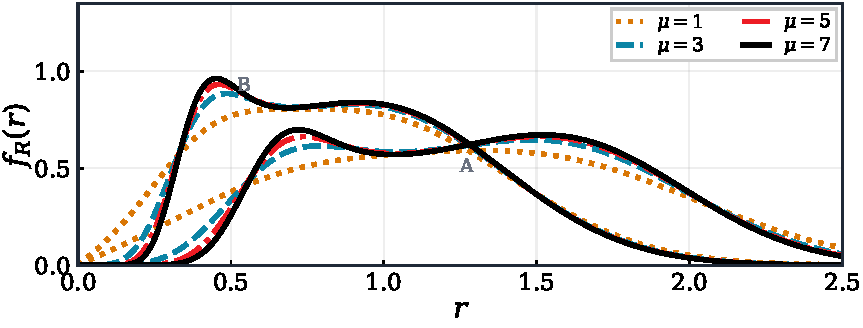
\includegraphics[width=0.78\linewidth]{figures/mftr_shape.pdf}
            \par}
        \noindent\makebox[\linewidth][c]{\parbox{0.78\linewidth}{$f_R(r)$ for
                $\mu\in\{1,3,5,7\}$, two parameter sets A and B. Bimodality grows with $\mu$.}}
    }

    \block{Architecture}{%
        {\vspace{0.60cm}
            {\centering
                \makebox[\linewidth][c]{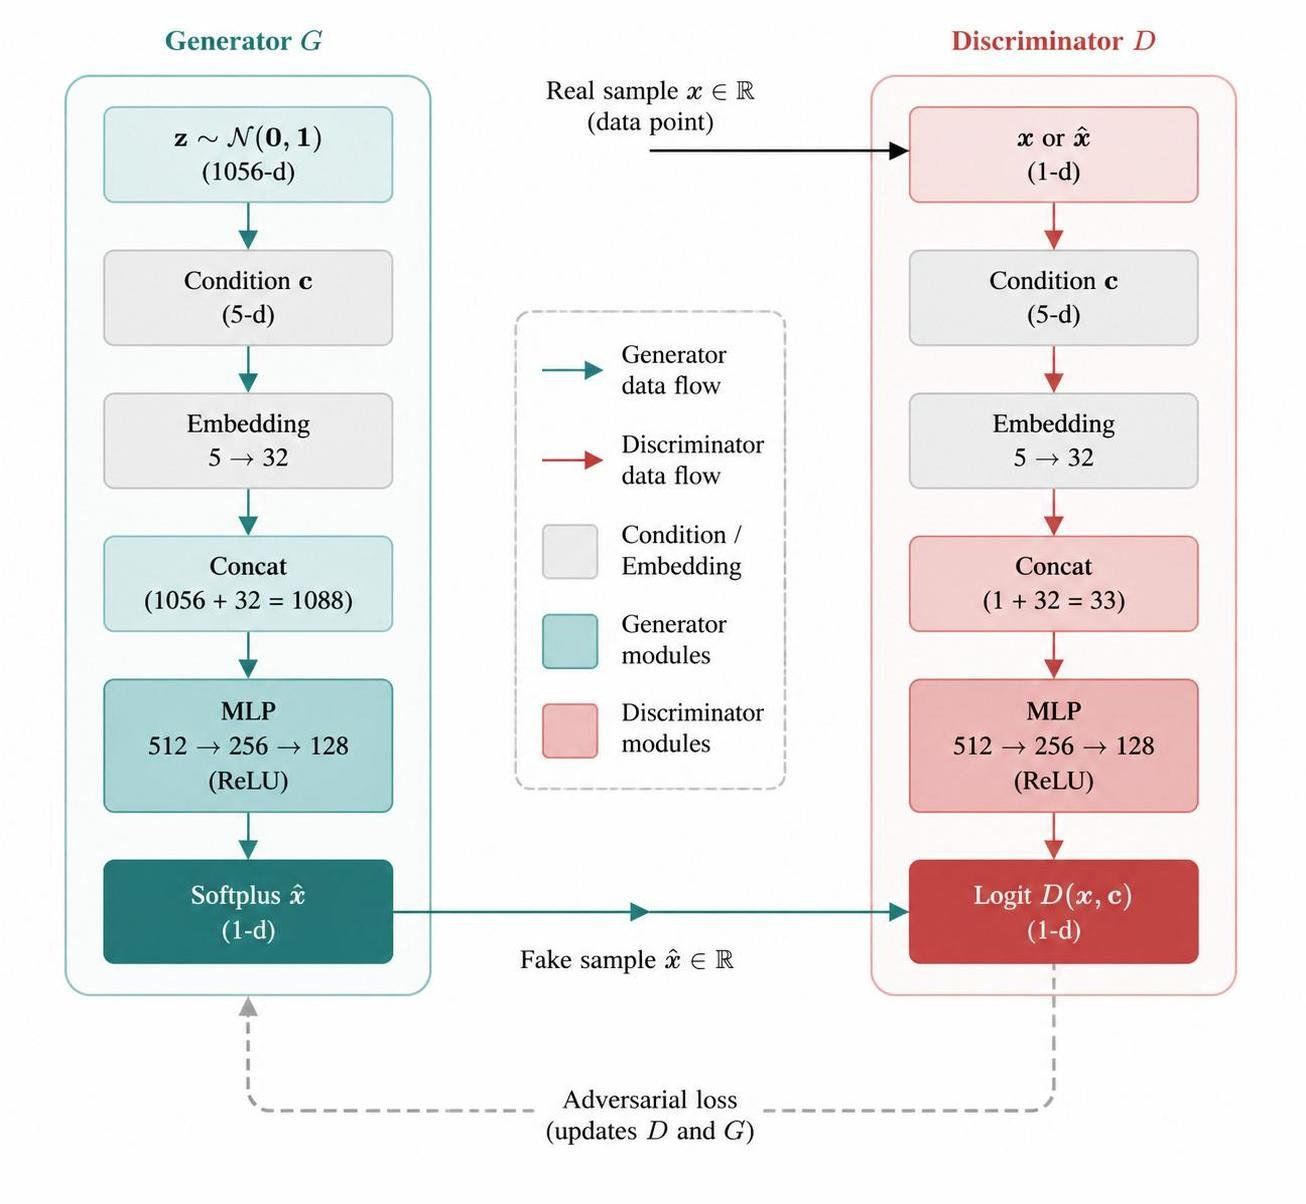
\includegraphics[width=0.7\linewidth]{figures/diagram.jpg}}
                \par}}

        \scriptsize
        Shared embedding: Linear--ReLU--Linear ($5\rightarrow32$),
        $\mathbf{c}$ normalized to $[-1,1]$.
        Adam $\beta_1=0.5$, lr$_G=2\times10^{-4}$, lr$_D=4\times10^{-4}$,
        batch 1024, update $G$ every 3 discriminator steps.
    }

    \block{Training Pipeline}{%
        {\vspace{0.55cm}
            {\centering
                \makebox[\linewidth][c]{\resizebox{0.80\linewidth}{!}{%
                        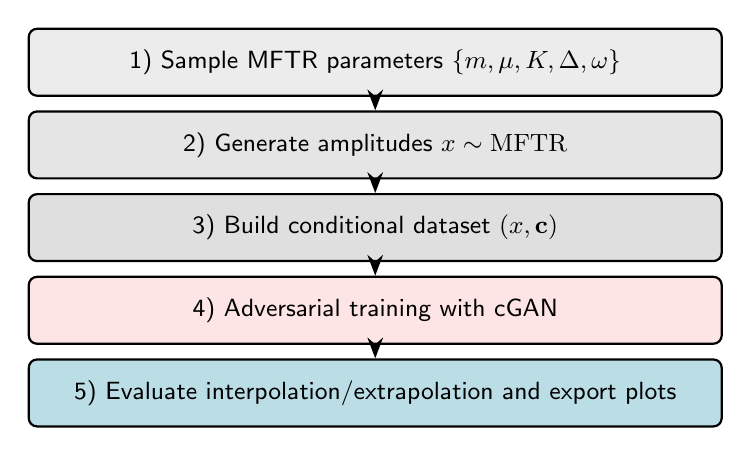
\begin{tikzpicture}[x=1cm,y=1cm]
                            \node[box, fill=gray!15, minimum width=8.8cm] (p1)
                            at (0,4.0) {1) Sample MFTR parameters $\{m,\mu,K,\Delta,\omega\}$};
                            \node[box, fill=gray!20, minimum width=8.8cm] (p2)
                            at (0,2.95) {2) Generate amplitudes $x\sim\mathrm{MFTR}$};
                            \node[box, fill=gray!25, minimum width=8.8cm] (p3)
                            at (0,1.9) {3) Build conditional dataset $(x,\mathbf{c})$};
                            \node[box, fill=usfqred!12, minimum width=8.8cm] (p4)
                            at (0,0.85) {4) Adversarial training with cGAN};
                            \node[box, fill=genteal!28, minimum width=8.8cm] (p5)
                            at (0,-0.2) {5) Evaluate interpolation/extrapolation and export plots};

                            \draw[farr] (p1) -- (p2);
                            \draw[farr] (p2) -- (p3);
                            \draw[farr] (p3) -- (p4);
                            \draw[farr] (p4) -- (p5);
                        \end{tikzpicture}
                    }}
                \par}}

        % \scriptsize
        % $m\!\in\![1,8]$, $\mu\!\in\![1,9]$, $K\!\in\![0,20]$,
        % $\Delta\!\in\![0,0.9]$, $\omega\!\in\![1,2]$;
        % 100k combos $\times$ 1k samples.
    }

    %% ===== COL 2  46% ==========================================
    \column{0.5}

    \block{Results: Interp.\ vs.\ Extrap.}{%
        \vspace{0.10cm}
        % \scriptsize
        \textcolor{genteal}{\rule[0.4ex]{1.0em}{1.0pt}}~Gen.\ KDE\quad
        \textcolor{discored}{\rule[0.4ex]{1.0em}{1.0pt}}~MFTR PDF\quad
        \textcolor{genteal}{\raisebox{0.4ex}{\textendash\textendash\textendash}}~Gen.\ CDF\quad
        \textcolor{discored}{\rule[0.4ex]{1.0em}{1.0pt}}~MFTR CDF

        \vspace{0.06cm}

        % --- Vertical stack for better portrait distribution ---
        {\scriptsize\textbf{Interp.~1} $m\!=\!5,\;\mu\!=\!2,\;K\!=\!8$ \hfill
            \scriptsize unimodal, in-range\par}
        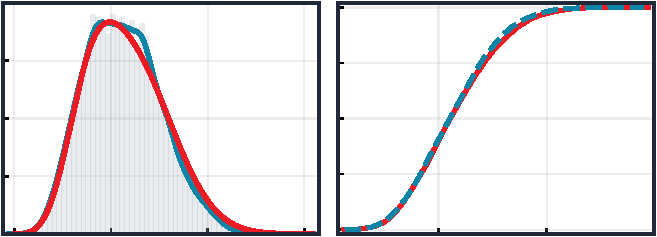
\includegraphics[width=0.80\linewidth]{figures/result_1.pdf}

        \vspace{0.02cm}
        {\scriptsize\textbf{Interp.~2} $m\!=\!6,\;\mu\!=\!7,\;K\!=\!12$ \hfill
            \scriptsize bimodal, in-range\par}
        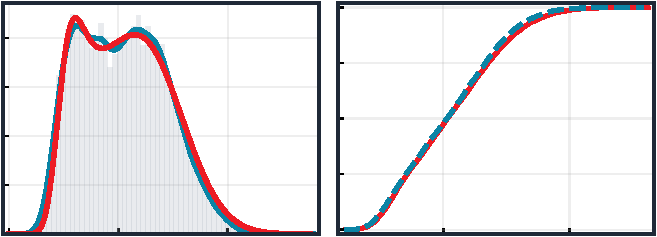
\includegraphics[width=0.80\linewidth]{figures/result_2.pdf}

        \vspace{0.02cm}
        {\scriptsize\textbf{Extrap.~1} $m\!=\!5,\;\bm{\mu}\!=\!12,\;K\!=\!8$ \hfill
            \scriptsize\textcolor{discored}{$\mu>9$ out-of-range}\par}
        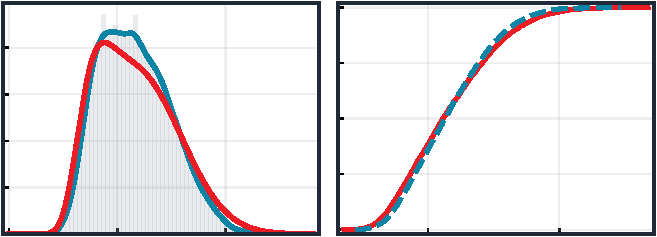
\includegraphics[width=0.80\linewidth]{figures/result_3.pdf}

        \vspace{0.02cm}
        {\scriptsize\textbf{Extrap.~2} $\bm{m}\!=\!10,\;\mu\!=\!5,\;K\!=\!8$ \hfill
            \scriptsize\textcolor{discored}{$m>8$ out-of-range}\par}
        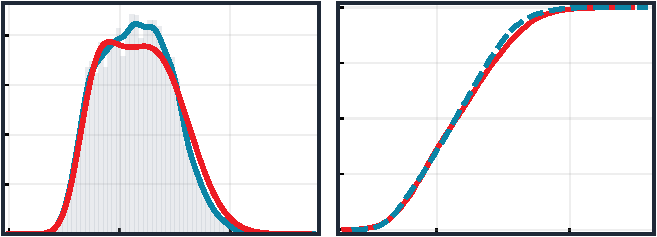
\includegraphics[width=0.80\linewidth]{figures/result_4.pdf}

        \vspace{0.03cm}
        % \scriptsize
        Each panel: \textbf{left} density (hist.\ + KDE + MFTR PDF),
        \textbf{right} empirical CDF.
        Interp.\ matches theory closely across unimodal and bimodal shapes.
        Extrap.\ degrades gracefully: similar median but larger
        worst-case errors (Wasserstein $\approx\!0.11$ vs.\ $\approx\!0.05$).
    }

    \block{Next Steps}{%
        \vspace{0.10cm}
        % \scriptsize
        Prioritized next step: transfer the full pipeline to
        \textbf{real wireless measurements}.

        \vspace{0.04cm}
        Six empirical scenarios with MFTR fitted parameters are ready.
        This poster prioritizes model behavior and synthetic-to-theory agreement.

        \vspace{0.04cm}
        {\centering
            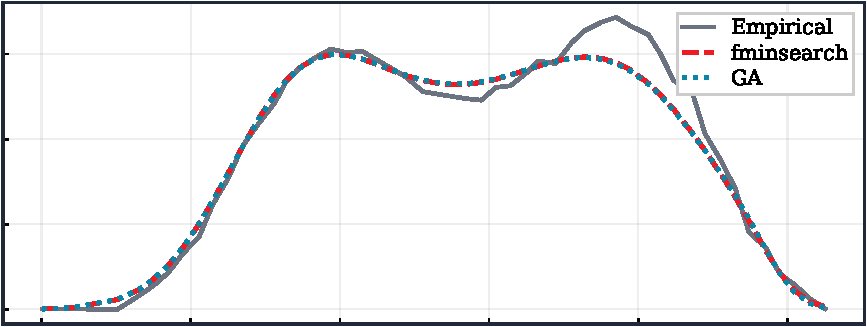
\includegraphics[width=0.74\linewidth]{figures/scenario1.pdf}
            \par}
        \vspace{0.03cm}
        Scenario~1: empirical (\textcolor{gray!60}{---}),
        fminsearch (\textcolor{discored}{--}), GA (\textcolor{genteal}{$\cdots$}).
    }


\end{columns}
\end{document}
